%%
%% Information Sciences (Elsevier) — LaTeX SINGLE-COLUMN submission template
%% - Single-column layout (Word requires single-column; LaTeX can be either, but you asked single-column)
%% - MANUAL bibliography (thebibliography) ✅  (NO .bib / BibTeX)
%% - Keeps your packages, tables, algorithms, and overall structure
%%

\documentclass[preprint,12pt]{elsarticle}

% -----------------------------
% Citations (author-year)
% -----------------------------

% -----------------------------
% Core packages (same as yours)

% -----------------------------
\usepackage{graphicx}
\usepackage{amsmath,amssymb,amsfonts}
\usepackage{xcolor}
\usepackage{url}
% ---------- Tables ----------
% ---------- Tables ----------
\usepackage{booktabs}
\usepackage{array}
\usepackage{multirow}
\usepackage[table]{xcolor}
\usepackage{makecell}
\usepackage{threeparttable}

% optional helpers
\newcommand{\best}[1]{\textbf{#1}}
\definecolor{tablehead}{gray}{0.92}
\definecolor{tablerow}{gray}{0.97}

% ---------- Algorithms ----------
\usepackage{algorithm}
\usepackage{algorithmicx}
\usepackage{algpseudocode}

% ---------- Misc ----------
\usepackage{threeparttable}
\raggedbottom


\journal{Knowledge-Based Systems}

\begin{document}

% \linenumbers % (Optional) enable if lineno is used above

\begin{frontmatter}

% -----------------------------
% Title
% -----------------------------
\title{MADiff-T: Multi-Agent Evolutionary Calibration of Diffusion Models for Privacy-Audited Tabular Data Generation}

% -----------------------------
% Authors / Affiliations (elsarticle style)


\author[aff1]{Kumail Javaid}
\author[aff1]{Yukang Cui\corref{cor1}}

\cortext[cor1]{Corresponding author. Email: cuiyukang@szu.edu.cn}

\address[aff1]{College of Mechatronics and Control Engineering, Shenzhen University, Shenzhen, China}

% -----------------------------
% Abstract
% -----------------------------
\begin{abstract}
Tabular synthetic data generation is challenging due to heterogeneous feature types, complex dependencies, and privacy risks arising from memorization. While GAN- and VAE-based generators are widely used, they can exhibit training instability and may leak information under attack-based audits. Denoising diffusion models offer a more stable alternative with strong fidelity, but their performance on tabular data is highly sensitive to calibration choices (e.g., noise schedule, step budget, and feature scaling) and single-model tuning can converge to suboptimal utility--privacy operating points.

We propose \textbf{MADiff-T}, a \textbf{multi-agent evolutionary refinement} framework for tabular diffusion. MADiff-T trains a population of diffusion ``agents'' that explore diffusion-specific calibration variables and applies elitist selection with mutation and weight inheritance. Selection is guided by a composite, \emph{privacy-audited} fitness that combines (i) downstream utility measured by Train-on-Synthetic, Test-on-Real (TSTR), (ii) lightweight marginal-alignment proxies, and (iii) in-loop privacy audits based on proximity (DCR) and a distance-based membership inference AUROC.

Across five real-world tabular benchmarks, MADiff-T improves TSTR utility over the original single-agent TabDDPM baseline on four of five datasets, although some gains are modest relative to seed variance, while shifting the utility--privacy operating point through privacy-in-the-loop selection. We further introduce two training enhancements: (i) a \textbf{Feature-Aggregated (FA) Loss} that re-weights continuous and categorical loss terms by per-feature inverse variance and inverse entropy, preventing high-variance features from monopolizing gradient signal, and (ii) \textbf{Per-Feature Schedule (PFS) offsets} that extend the evolutionary search to per-feature noise schedule perturbations, with adaptive activation based on dataset size and feature-type composition. Together these enhancements improve TSTR by up to $+$12.2 percentage
points over the single-agent TabDDPM baseline on Heart, with more modest gains on other datasets. Importantly, MADiff-T uses multi-agent refinement only during training; deployment uses a single selected model. All privacy results are \emph{audit-based} under stated protocols and do not constitute a formal differential privacy guarantee.
\end{abstract}

% -----------------------------
% Highlights (encouraged by Elsevier)
% -----------------------------
\begin{highlights}
\item Multi-agent evolutionary calibration of tabular diffusion with in-loop privacy audits (DCR + MIA-AUC).
\item Feature-Aggregated Loss with per-feature inverse-variance and inverse-entropy weighting and adaptive $\lambda_{\text{cat}}$.
\item Per-Feature Schedule offsets evolved as calibration variables with adaptive dataset-size-based activation.
\item TSTR improvements on four of five benchmarks (up to $+$12.2pp
vs single-agent TabDDPM on Heart) with improved privacy operating points.
\end{highlights}

% -----------------------------
% Keywords (1–7 recommended)
% -----------------------------
\begin{keyword}
Synthetic data \sep Tabular data \sep Diffusion models \sep Evolutionary optimization \sep Privacy auditing \sep Membership inference
\end{keyword}

\end{frontmatter}

% ==========================================================
% MAIN TEXT (PASTE YOUR EXISTING SECTIONS UNCHANGED BELOW)
% ==========================================================

\section{Introduction}
Synthetic tabular data is increasingly used to enable data sharing and model development when direct access to sensitive records is restricted \cite{Kindji2025}. Recent syntheses of the field emphasize that tabular synthetic data is now evaluated under tighter expectations around downstream utility, privacy risk, and reproducibility \cite{cormode2025synthetic_tabular_kdd}. In regulated domains, synthetic data is sometimes positioned as an anonymisation technique, yet legal and adversarial scrutiny of ``anonymised'' releases is tightening \cite{Pilgram2025}. In parallel, privacy research has shown that learning systems can leak information about individuals through membership inference and related attacks \cite{Shokri2017}.

Deep generative models are a dominant approach for tabular synthesis because they can capture high-dimensional dependencies that classical simulators often fail to preserve \cite{Kindji2025}. Early successes include GAN and VAE formulations \cite{Goodfellow2014}. Tabular-specialised variants improve mixed-type handling and downstream utility through conditioning and tailored preprocessing \cite{Xu2019a}. However, strong utility can coincide with overfitting and privacy leakage, and training stability remains challenging in low-data regimes \cite{Alaa2022}. Differential privacy provides formal guarantees in principle \cite{Dwork2014}, but practical DP training can degrade utility and requires careful tuning of privacy budgets and optimisation hyperparameters \cite{Abadi2016}.

Diffusion models have recently emerged as a competitive alternative for tabular generation due to stable likelihood-based training and improved mode coverage \cite{Kotelnikov2023}. Latent-space score-based synthesis for mixed-type tabular data further improves sampling efficiency and performance across benchmarks \cite{Zhang2024}. Diffusion-based generators have also been explored in sensitive health settings where reliability and privacy are central concerns \cite{Tian2024}. A recurring limitation is that tabular diffusion performance is highly sensitive to calibration choices such as noise schedules and step budgets \cite{karras2022edm_neurips}. Feature-wise scaling and preprocessing decisions can further shift the operating point, especially under mixed-type constraints \cite{VillaizanVallelado2025}.

Despite these advances, privacy is still commonly treated as a post-hoc audit rather than a first-class selection signal during model calibration \cite{Hernandez2025}. To address this gap, we propose MADiff-T (Multi-Agent Diffusion for Tabular data), a multi-agent evolutionary refinement framework that calibrates tabular diffusion generators under a privacy-audited objective. Related multi-agent generators such as HydraGAN optimize multiple objectives via cooperative agents, but are not designed to calibrate diffusion processes with privacy auditing embedded directly into the selection loop \cite{DeSmetCook2024}. Evolutionary optimisation provides practical mechanisms for searching non-convex hyperparameter spaces \cite{Back1996,Hansen2001}, yet diffusion-specific calibration for mixed-type tabular synthesis with privacy-in-the-loop selection remains underexplored. Compared to generic population-based tuning, MADiff-T explicitly optimises diffusion calibration variables (noise schedule, step budget, and feature-wise scaling) and uses weight inheritance to traverse the calibration space without full retraining.

Concretely, MADiff-T maintains a population of diffusion agents trained with diverse calibration settings and periodically refines the population via elitist selection, mutation, and weight inheritance. In selection, we use DCR-based proximity as a primary \emph{but not sufficient} privacy signal \cite{yao2025dcr_delusion}. We also use a distance-based membership inference AUROC (MIA AUC) as a second primary privacy signal \cite{Hayes2019,ZhangMalin2022}. Authenticity-style sample-level indicators are reported as secondary audits for transparency \cite{Alaa2022}. Importantly, our privacy claims are audit-based under stated threat models rather than a formal DP guarantee \cite{lautrup2025syntheval}. The multi-agent mechanism is a training strategy: deployment uses a single selected refined diffusion model rather than an ensemble.

Our main contributions are:
\begin{itemize}
    \item We introduce \textbf{MADiff-T}, a \textbf{multi-agent evolutionary calibration} framework for tabular diffusion models that jointly targets fidelity, downstream utility, and privacy auditing during refinement, with weight inheritance enabling efficient calibration search without full retraining.
    \item We propose a \textbf{privacy-audited fitness} for evolutionary selection that explicitly incorporates DCR-based proximity and MIA resistance, separated from metrics reported only at evaluation time to avoid metric overfitting \cite{Hernandez2025}.
    \item We introduce a \textbf{Feature-Aggregated (FA) Loss} that applies per-feature inverse-variance weighting for continuous features and per-feature inverse-entropy weighting for categorical features, with a dataset-adaptive categorical loss coefficient $\lambda_{\text{cat}}$ that scales automatically with the continuous-to-categorical feature ratio.
    \item We introduce \textbf{Per-Feature Schedule (PFS) offsets}, extending the evolutionary calibration variables to include per-feature noise schedule perturbations with an adaptive activation rule based on training set size and feature-type composition.
   \item We provide extensive empirical evaluation across five benchmarks 
spanning small- to medium-scale regimes, with ablations isolating each 
contribution and contextualising results against the broader landscape 
of differentially private tabular synthesis 
\cite{chen2025benchmarking_dp_tabular_synthesis}.
\end{itemize}
The remainder of the paper reviews related work on tabular synthesis, diffusion modelling, and privacy evaluation; details the MADiff-T methodology and fitness design; and reports experiments and ablations that isolate the impact of multi-agent refinement and privacy-in-the-loop calibration.

\section{Related Work}\label{sec:related}
We review prior work on synthetic tabular data generation, diffusion models for structured data, population-based optimisation for generative modelling, and privacy auditing protocols for synthetic data \cite{cormode2025synthetic_tabular_kdd}.

\subsection{Synthetic Tabular Data Generation}\label{sec:rw_tabular}
Synthetic tabular data generation is widely studied as a mechanism to support data sharing and downstream modelling when access to real records is restricted \cite{Kindji2025}. Surveys and benchmarks emphasise that tabular synthesis should be evaluated jointly across utility, fidelity, and privacy rather than a single score \cite{lautrup2024systematic_review_tabular_synthesis_csur}. In practice, GAN and VAE baselines remain common for tabular synthesis, particularly conditional formulations designed for mixed feature types and imbalanced categories \cite{Xu2019a}. Subsequent variants improve mixed-type handling and robustness through architectural and preprocessing refinements \cite{zhao2022ctabganplus_frontiers}. Recent work increasingly incorporates task-aware or task-guided objectives, where the generator is evaluated through downstream learning performance \cite{Jia2024}.

A key takeaway from recent benchmarking and tuning studies is that reported performance can vary substantially with preprocessing, hyperparameters, and evaluation choices \cite{Restrepo2025}. This motivates refinement strategies that search calibration settings efficiently while keeping evaluation aligned with utility and privacy needs \cite{Kindji2025}.

\subsection{Diffusion Models for Tabular and Health Data}\label{sec:rw_diffusion}
Diffusion models have emerged as strong candidates for high-fidelity tabular synthesis, offering stable training and broad mode coverage compared with adversarial objectives \cite{Kotelnikov2023}. Latent-space score/diffusion approaches for mixed-type synthesis such as TabSyn provide an alternative design that improves sampling efficiency while maintaining competitive quality \cite{Zhang2024}. Beyond generic tabular datasets, diffusion models have also been explored in privacy-sensitive health settings where reliability and privacy are central concerns \cite{Tian2024}. Alternative score-based approaches for structured data generation further support the trend that score/diffusion paradigms can be effective for complex tabular distributions \cite{Kim2023}.

However, diffusion performance on tabular data can be sensitive to calibration choices such as noise schedule design and timestep budgets \cite{karras2022edm_neurips}. Recent syntheses highlight that calibration and preprocessing decisions can dominate performance differences across methods \cite{VillaizanVallelado2025}. These observations motivate approaches that treat diffusion calibration as an explicit search problem rather than a fixed, one-shot configuration \cite{Kotelnikov2023}.

\subsection{Cooperative and Evolutionary Optimisation for Generative Modelling}\label{sec:rw_multiagent}
Cooperative and population-based approaches have been explored to improve generative modelling under multiple objectives. HydraGAN provides a representative example of cooperative multi-objective generation via multiple agents \cite{DeSmetCook2024}. Separately, evolutionary computation has been surveyed as a mechanism to improve GAN training dynamics and model selection \cite{Wang2024EvolutionaryGAN}. 
These works support the broader idea that population-level optimisation can be effective 
when objectives compete and the search space is non-convex \cite{Back1996,Hansen2001}. 
Automated machine learning and neural architecture search have similarly applied 
population-based strategies to model selection and hyperparameter search across 
a range of learning tasks \cite{He2021AutoML}. However, these frameworks are not 
designed for diffusion-specific calibration variables nor do they incorporate 
privacy-audited objectives directly into the selection loop.

In tabular synthesis benchmarks, model selection is often conducted via multi-run tuning without explicit weight inheritance \cite{Restrepo2025}. This increases cost when exploring calibration spaces, especially for diffusion models with expensive training and sampling loops \cite{VillaizanVallelado2025}. Diffusion-specific calibration for mixed-type tabular synthesis under privacy-audited selection remains comparatively underexplored \cite{Hernandez2025}.

\subsection{Privacy Auditing and Evaluation for Synthetic Tabular Data}\label{sec:rw_privacy}
A growing body of work shows that synthetic data can leak information about training records under realistic threat models \cite{ZhangMalin2022}. Membership inference and overfitting-based audits have been demonstrated against synthetic data generators in tabular and health settings \cite{vanbreugel2023domias_aistats}. Re-identification and attack studies also show that vulnerabilities can persist even when utility metrics look strong \cite{Alshantti2025}. As a result, privacy evaluation is increasingly treated as an essential component of synthetic data reporting, alongside fidelity and utility \cite{lautrup2025syntheval}.

Recent evaluation frameworks formalise auditing protocols and encourage reporting under explicit threat models \cite{Hyrup2025}. Practical toolchains aim to operationalise privacy testing and reporting for synthetic tabular releases \cite{houssiau2022tapas}. Survey work consolidates these methods and highlights gaps in how audits are applied in practice \cite{hu2022membership_inference_survey}. Legal scrutiny of synthetic data releases further motivates rigorous evaluation and transparent privacy reporting \cite{Pilgram2025}. In this paper, we distinguish between \emph{privacy audits used for selection} versus \emph{audits reported as secondary diagnostics} (details in Section~\ref{sec:method}).

\subsection{Positioning of MADiff-T}\label{sec:rw_positioning}
Building on these foundations, we propose MADiff-T, a multi-agent evolutionary refinement framework for tabular diffusion models. Our goal is not to introduce a new diffusion architecture, but to provide a training-time refinement strategy that navigates diffusion calibration choices while explicitly accounting for privacy risk \cite{Hernandez2025}.

Compared to generic population-based tuning, MADiff-T optimises diffusion-specific calibration variables (noise schedule, step budget, and feature-wise scaling) under a privacy-audited fitness, and uses weight inheritance to traverse the calibration space without full retraining.

HydraGAN is an important reference point for cooperative multi-objective generation \cite{DeSmetCook2024}. In contrast, MADiff-T is designed specifically for diffusion calibration with privacy-audited selection and weight inheritance, and the multi-agent mechanism is used only during training while deployment uses a single selected model. To avoid ``metric soup,'' we separate metrics used in the optimisation loop from those used for reporting. In selection, we use DCR-style proximity and a distance-based membership inference AUROC as primary privacy signals \cite{yao2025dcr_delusion,Hayes2019,ZhangMalin2022}. Additional authenticity-style indicators and broader auditing toolchains are reported as secondary diagnostics for transparency \cite{Alaa2022,lautrup2025syntheval}.



\section{Methodology}
\label{sec:method}

\subsection{Problem setup and overview}
Let $D=\{(\mathbf{x}^{(n)}, y^{(n)})\}_{n=1}^{N}$ denote a tabular dataset of $N$ records, where $\mathbf{x}\in\mathbb{R}^{d_c}\times\mathcal{C}_1\times\cdots\times\mathcal{C}_{d_d}$ contains $d_c$ continuous features and $d_d$ categorical features, and $y$ is an optional downstream label. We split $D$ into $D_{\text{train}},D_{\text{val}},D_{\text{test}}$. All generators are trained only on $D_{\text{train}}$, in-loop utility and privacy signals used for evolutionary selection are computed using $D_{\text{val}}$ (to avoid test leakage), and $D_{\text{test}}$ is used only once for final reporting \cite{Hernandez2025}. When labels are available, we model the joint distribution $p(\mathbf{x},y)$ by treating $y$ as an additional categorical column during generation; however, all distance-based privacy audits below compute distances using $\mathbf{x}$ only (the label column is excluded from distance calculations) \cite{Hyrup2025}.

\paragraph{Why privacy-in-the-loop rather than post-hoc?}
A natural alternative to privacy-in-the-loop selection is to 
train a generator optimising utility alone and audit privacy 
post-hoc, discarding models that fail the audit threshold. 
This approach has two fundamental limitations. First, 
post-hoc rejection wastes training compute: a model trained 
to maximise utility may systematically converge toward 
high-memorisation regions of the calibration space that 
a privacy audit would reject, meaning most candidates are 
discarded late. Second, post-hoc auditing provides no signal 
to guide the calibration search away from unsafe regions. 
By contrast, incorporating privacy signals directly into 
the evolutionary fitness function steers the population 
toward calibrations that jointly satisfy utility and privacy 
constraints from the first generation, exploiting the 
structure of the calibration space rather than treating 
privacy as an external filter \cite{Hernandez2025,Hyrup2025}.

We propose MADiff-T (\underline{M}ulti-\underline{A}gent \underline{Diff}usion for \underline{T}abular data): a training-time, population-based refinement strategy that calibrates a tabular diffusion generator by evolving a population of diffusion ``agents'' under a privacy-audited fitness. The multi-agent component is used only during training, deployment uses a single selected model. MADiff-T searches diffusion-specific calibration variables, including noise schedule family/shape, step budget, and feature-wise scaling, and selects agents using explicit privacy audits in the loop (Section~\ref{sec:method_fitness}).

\begin{figure*}[!htpb]
    \centering \includegraphics[width=\linewidth]{figures/fig_madifft_overview.pdf}
    \caption{Overview of MADiff-T. A population of tabular diffusion agents is trained and evaluated each generation. Elites are selected by a composite fitness that includes in-loop privacy audits (DCR proximity and a distance-based membership inference proxy AUC computed with $D_{\text{val}}$ as non-members). New agents are created via mutation of diffusion calibration variables with weight inheritance. Deployment uses the best single selected model.}
    \label{fig:madifft_overview}
\end{figure*}

\subsection{Tabular diffusion backbone}
MADiff-T can be applied to tabular diffusion generators; in this work we use a TabDDPM-style mixed-type diffusion backbone \cite{Kotelnikov2023}. Continuous features are standardized using statistics from $D_{\text{train}}$ (and optionally transformed monotonically, e.g., quantile). Categorical features are represented consistently with the backbone implementation (e.g., indices or one-hot). Let $\mathbf{z}_0$ denote the resulting model-space vector.

\paragraph{Forward noising (continuous part)}
For continuous features, the forward diffusion process adds Gaussian noise over $T$ steps:
\begin{equation}
q(\mathbf{z}_t \mid \mathbf{z}_{t-1}) = \mathcal{N}\!\left(\sqrt{1-\beta_t}\,\mathbf{z}_{t-1},\, \beta_t \mathbf{I}\right), \quad t=1,\dots,T,
\end{equation}
with noise schedule $\{\beta_t\}_{t=1}^{T}$. Defining $\alpha_t=1-\beta_t$ and $\bar{\alpha}_t=\prod_{s=1}^{t}\alpha_s$, we obtain:
\begin{equation}
q(\mathbf{z}_t \mid \mathbf{z}_0) = \mathcal{N}\!\left(\sqrt{\bar{\alpha}_t}\,\mathbf{z}_0,\, (1-\bar{\alpha}_t)\mathbf{I}\right).
\end{equation}

\paragraph{Discrete corruption (categorical part)}
For categorical columns, we use random-replacement corruption: at each noising step $t$, each categorical entry is replaced by a uniformly sampled category from its column domain with probability
\begin{equation}
\gamma_t = \frac{t}{T}, \qquad t=1,\dots,T,
\end{equation}
and kept unchanged with probability $1-\gamma_t$. This is consistent with mixed-type diffusion designs for tabular synthesis and structured diffusion in discrete state-spaces \cite{Kotelnikov2023,Austin2021}.

\paragraph{Reverse model and objective}
The reverse process is parameterized by a network $f_{\theta}$ that conditions on time $t$ (via a time embedding) and predicts (i) continuous noise (or denoised signal) and (ii) categorical logits. We use a noise-prediction objective for continuous features and cross-entropy for categorical features:
\begin{equation}
\mathcal{L}(\theta)=
\mathbb{E}_{t,\mathbf{z}_0,\boldsymbol{\epsilon}}\left[\left\|\boldsymbol{\epsilon}-f_{\theta}^{(c)}(\mathbf{z}_t,t)\right\|_2^2\right]
\;+\;
\lambda_{\text{cat}} \cdot
\mathbb{E}_{t,\mathbf{z}_0}\left[\mathrm{CE}\!\left(\mathbf{x}^{(d)},\, f_{\theta}^{(d)}(\mathbf{z}_t,t)\right)\right].
\label{eq:diff_loss}
\end{equation}
To sample synthetic records, we start from $\mathbf{z}_T$ (Gaussian noise for continuous features and maximally corrupted categories), apply learned reverse transitions to obtain $\mathbf{z}_0$, then invert preprocessing to return to the original feature space.

\subsection{MADiff-T: population refinement with weight inheritance}
MADiff-T maintains a population of $M$ diffusion agents at generation $g$:
\begin{equation}
\mathcal{P}^{(g)}=\left\{A_i^{(g)}=(\theta_i^{(g)},\, h_i^{(g)})\right\}_{i=1}^{M},
\end{equation}
where $\theta_i$ are network weights and $h_i$ is a vector of diffusion calibration variables. To keep weight inheritance exact, the backbone architecture is fixed and is not mutated. In this work, $h_i$ includes: (i) noise schedule family/shape (linear/cosine/sigmoid and a shape scalar), (ii) step budget $T$, (iii) a global $\beta$-scale, (iv) feature-wise scaling for continuous columns (post-sampling dispersion correction), and (v) dropout.

Each generation uses a fixed per-agent training budget of $B$ optimizer steps:
\begin{enumerate}
    \item Train each agent on $D_{\text{train}}$ for $B$ steps under its calibration $h_i^{(g)}$ by minimizing Eq.~\eqref{eq:diff_loss}.
    \item Generate a synthetic dataset $\tilde{D}_i^{(g)}$ with $|\tilde{D}_i^{(g)}|=|D_{\text{train}}|$.
    \item Score $\tilde{D}_i^{(g)}$ via a composite fitness (Section~\ref{sec:method_fitness}) that includes in-loop privacy audits.
\end{enumerate}
Agents are ranked by fitness, the top $K$ elites are retained, and the remaining $M-K$ agents are replaced by offspring. Offspring are created by mutating calibration variables and inheriting weights:
\begin{equation}
h_{\text{child}} \leftarrow \mathrm{Mutate}(h_{\text{parent}}),
\qquad
\theta_{\text{child}} \leftarrow \theta_{\text{parent}}.
\end{equation}

Unlike generic population training that primarily perturbs optimiser settings, MADiff-T optimises diffusion-specific calibration variables (noise schedule, step budget, feature-wise scaling) under a privacy-audited fitness and uses weight inheritance to traverse the calibration space without full retraining.

We position MADiff-T relative to cooperative multi-agent generators (e.g., HydraGAN) and evolutionary optimisation principles \cite{Back1996,Hansen2001}.

\begin{algorithm}[H]
\caption{MADiff-T: Multi-Agent Evolutionary Refinement for Tabular Diffusion}
\label{alg:madifft}
\footnotesize
\begin{algorithmic}[1]
\Require $D_{\text{train}},D_{\text{val}}$; population $M$; elites $K$; generations $G$; per-agent budget $B$; search space $\mathcal{H}$
\Ensure Best refined agent $A^\star$
\State Initialize $\mathcal{P}^{(1)}=\{(\theta_i^{(1)}, h_i^{(1)})\}_{i=1}^{M}$ with $h_i^{(1)}\sim\mathcal{H}$
\For{$g \gets 1$ to $G$}
    \For{$i \gets 1$ to $M$}
        \State Train $A_i^{(g)}$ on $D_{\text{train}}$ for $B$ steps using $h_i^{(g)}$
        \State Sample $\tilde{D}_i^{(g)} \sim p_{\theta_i^{(g)}}(\cdot \mid h_i^{(g)})$
        \State $S_i^{(g)} \leftarrow \mathrm{Fitness}(\tilde{D}_i^{(g)};\,D_{\text{train}},D_{\text{val}})$
    \EndFor
    \State $\mathcal{E}^{(g)} \leftarrow$ top-$K$ agents in $\mathcal{P}^{(g)}$ by $S_i^{(g)}$
    \State $\mathcal{P}^{(g+1)} \leftarrow \mathcal{E}^{(g)}$
    \While{$|\mathcal{P}^{(g+1)}| < M$}
        \State Sample parent $(\theta_p, h_p) \in \mathcal{E}^{(g)}$
        \State $h_{\text{child}} \leftarrow \mathrm{Mutate}(h_p)$
        \State $\theta_{\text{child}} \leftarrow \theta_p$ \Comment{weight inheritance}
        \State Add $(\theta_{\text{child}}, h_{\text{child}})$ to $\mathcal{P}^{(g+1)}$
    \EndWhile
\EndFor
\State \Return $A^\star=\arg\max_{A_i^{(G)}\in \mathcal{P}^{(G)}} S_i^{(G)}$
\end{algorithmic}
\end{algorithm}
\subsection{Feature-Aggregated Loss}
\label{sec:method_faloss}

The standard tabular diffusion objective (Eq.~\ref{eq:diff_loss}) weights all continuous features equally and uses a fixed $\lambda_{\text{cat}}$ regardless of dataset composition. On heterogeneous tabular datasets, features with greater learning difficulty can dominate the reconstruction loss while categorical features may be undertrained when $\lambda_{\text{cat}}$ is set without reference to the actual feature ratio. We use inverse empirical variance as a practical proxy for per-feature difficulty: features with larger variance contribute more raw MSE and disproportionately influence gradient magnitude, so down-weighting them rebalances the optimization across heterogeneous continuous columns. We address both issues with the Feature-Aggregated (FA) Loss.

\paragraph{Per-feature continuous weights}
Let $\sigma_k^2$ denote the empirical variance of continuous feature $k$ computed from $D_{\text{train}}$. We define inverse-variance importance weights:
\begin{equation}
w_k^{(c)} = \frac{1/\sigma_k^2}{\sum_{j=1}^{d_c} 1/\sigma_j^2}, \quad k = 1, \dots, d_c,
\label{eq:fa_cont_weights}
\end{equation}
clipped to $[0.5, 2.0]$ before normalization to prevent extreme ratios. The weighted continuous loss becomes:
\begin{equation}
\mathcal{L}_{\text{cont}}(\theta) = \sum_{k=1}^{d_c} w_k^{(c)} \cdot \mathbb{E}_{t, \mathbf{z}_0, \boldsymbol{\epsilon}}\!\left[\left(\epsilon_k - f_{\theta,k}^{(c)}(\mathbf{z}_t, t)\right)^2\right].
\label{eq:fa_cont_loss}
\end{equation}

\paragraph{Per-feature categorical weights.}
Let $H_j = -\sum_v p_{jv} \log p_{jv}$ denote the empirical entropy of categorical feature $j$ in $D_{\text{train}}$. We use inverse entropy as a heuristic weighting signal, with the intuition that low-entropy (highly skewed) categorical features have tighter acceptable-output distributions and benefit from relatively more gradient pressure to avoid mode collapse onto the majority class. This is a heuristic, not a theoretical guarantee; we ablate its contribution in Section~\ref{sec:ablation}.
\begin{equation}
w_j^{(d)} = \frac{1/(H_j + \varepsilon)}{\sum_{l=1}^{d_d} 1/(H_l + \varepsilon)}, \quad j = 1, \dots, d_d, \quad \varepsilon = 10^{-8}.
\label{eq:fa_cat_weights}
\end{equation}

\paragraph{Adaptive $\lambda_{\text{cat}}$.}
Rather than fixing $\lambda_{\text{cat}} = 0.5$ regardless of dataset composition, we compute:
\begin{equation}
\lambda_{\text{cat}} = \min\!\left(0.85,\; 0.3 + 0.5 \cdot \frac{d_d}{d_c + d_d}\right),
\label{eq:auto_lambda}
\end{equation}
clipped to $[0.25, 0.85]$. This scales $\lambda_{\text{cat}}$ upward for predominantly categorical datasets and downward for purely continuous ones. The FA Loss replaces Eq.~\eqref{eq:diff_loss} in all agent training steps:
\begin{equation}
\mathcal{L}_{\text{FA}}(\theta) = \mathcal{L}_{\text{cont}}(\theta) + \lambda_{\text{cat}} \cdot \sum_{j=1}^{d_d} w_j^{(d)} \cdot \mathbb{E}_{t, \mathbf{z}_0}\!\left[\mathrm{CE}\!\left(x_j^{(d)},\, f_{\theta,j}^{(d)}(\mathbf{z}_t, t)\right)\right].
\label{eq:fa_loss}
\end{equation}

\subsection{Per-Feature Schedule Offsets}
\label{sec:method_pfs}

The tabular diffusion backbone applies one global noise schedule $\{\beta_t\}$ identically to all continuous features. However, tabular features have heterogeneous noise sensitivities: nuclear texture measurements in medical datasets behave differently under Gaussian corruption than demographic features in income datasets. Motivated by per-feature schedule designs in recent diffusion work \cite{VillaizanVallelado2025}, we add lightweight per-feature schedule offsets to the evolutionary calibration variables.

\paragraph{Per-feature effective schedule.}
For each continuous feature $k$, we define:
\begin{equation}
\beta_t^{(k)} = \mathrm{clip}\!\left(\beta_t \cdot e^{\alpha_k} + \gamma_k,\; 10^{-5},\; 0.999\right),
\label{eq:pfs}
\end{equation}
where $\alpha_k \in [-0.15, 0.15]$ is a log-scale multiplier and $\gamma_k \in [-0.01, 0.01]$ is an additive offset, both stored in the agent calibration variables $h_i$. At initialization, $\alpha_k = \gamma_k = 0$ for all $k$, so Eq.~\eqref{eq:pfs} reduces to the global schedule exactly. The evolutionary search then discovers non-zero offsets across generations. The reverse network $f_\theta$ is unchanged; per-feature schedules affect only the forward noising process. Note that because each $\beta_t^{(k)}$ acts independently on feature $k$, the forward noising covariance remains diagonal in feature space: PFS perturbs per-feature variances but does not introduce cross-feature correlations in the noise process.

\paragraph{Adaptive activation.}
On datasets where the continuous subspace is too small for reliable per-feature search (specifically, $n_{\text{train}} < 520$ or $d_d/(d_c + d_d) \geq 0.5$), the offsets are frozen at zero throughout training, effectively degenerating to the global schedule. The training-size threshold (520) and the categorical-fraction threshold (0.5) are user-tunable hyperparameters; we use these values across all experiments but they can be adjusted for other data regimes. This prevents the evolutionary search from introducing instability on small or predominantly categorical datasets. Mutation of $\alpha_k$ and $\gamma_k$ perturbs approximately 30\% of features per mutation event with small Gaussian noise, consistent with the broader calibration mutation strategy.
\subsection{Composite fitness with in-loop privacy audits}
\label{sec:method_fitness}

MADiff-T ranks agents using a scalar fitness. To avoid ``metric soup'', we use only a small set of metrics in selection (utility, lightweight fidelity, and two privacy audits), while additional audits are reported only at evaluation time \cite{Hernandez2025,Hyrup2025}.

\paragraph{Mixed-type distance for audits.}
All proximity-based audits use a mixed-type distance on features $\mathbf{x}$ (excluding the label column). Let $\mathbf{x}=(\mathbf{x}^{(c)},\mathbf{x}^{(d)})$ denote continuous and categorical parts after preprocessing; $\mathbf{x}^{(c)}$ is z-scored using $D_{\text{train}}$ statistics and categorical values are compared by per-column equality. We define:
\begin{equation}
\mathrm{dist}(\mathbf{x},\mathbf{x}')=\alpha \cdot \frac{\left\|\mathbf{x}^{(c)}-\mathbf{x}'^{(c)}\right\|_2}{\sqrt{d_c}}
\;+\;
(1-\alpha)\cdot \frac{1}{d_d}\sum_{j=1}^{d_d}\mathbb{I}\!\left[x^{(d)}_j\neq x'^{(d)}_j\right],
\label{eq:mixdist}
\end{equation}
where the second term is normalized Hamming distance and $\alpha\in[0,1]$ balances continuous and categorical contributions (we use $\alpha=0.5$ unless stated otherwise). For datasets with only continuous features ($d_d=0$) the categorical term is omitted and we set $\alpha=1$; for datasets with only categorical features ($d_c=0$) the continuous term is omitted and we set $\alpha=0$, so Eq.~\eqref{eq:mixdist} is well-defined in all cases.

\paragraph{In-loop utility and fidelity.}
Utility is computed as TSTR on validation: a predictor is trained on $\tilde{D}$ and evaluated on $D_{\text{val}}$, yielding $U(\tilde{D})\in[0,1]$ \cite{Jia2024}. Fidelity $F(\tilde{D},D_{\text{train}})\in[0,1]$ is computed via lightweight distribution proxies (e.g., mean/std deviations for continuous features and marginal divergence for categoricals) to keep selection computationally cheap.

\paragraph{In-loop privacy audits.}
We use two audits:
\begin{itemize}
    \item \textbf{DCR proximity (low quantile).} Define
    \begin{equation}
    \mathrm{DCR}_{q}(\tilde{D},D_{\text{train}})=
    \mathrm{Quantile}_{q}\left(\left\{\min_{\mathbf{x}\in D_{\text{train}}}\mathrm{dist}(\tilde{\mathbf{x}},\mathbf{x}) : \tilde{\mathbf{x}}\in \tilde{D}\right\}\right),
    \end{equation}
    with a low quantile (e.g., $q=0.01$). For stable ranking across generations, we compute a normalized variant by dividing by within-real leave-one-out nearest-neighbor distances (excluding identical records):
   \begin{equation}
\begin{aligned}
\mathrm{DCR}_{q}^{\mathrm{LOO}}(D_{\text{train}})
&=
\mathrm{Quantile}_{q}\!\Big(
\Big\{
\min_{\mathbf{x}'\in D_{\text{train}}\setminus\{\mathbf{x}\}}
\mathrm{dist}(\mathbf{x},\mathbf{x}')
:\mathbf{x}\in D_{\text{train}}
\Big\}
\Big).
\end{aligned}
\end{equation}

    \begin{equation}
    \mathrm{NormDCR}(\tilde{D},D_{\text{train}})=
    \frac{\mathrm{DCR}_{q}(\tilde{D},D_{\text{train}})}{\mathrm{DCR}_{q}^{\mathrm{LOO}}(D_{\text{train}})+\varepsilon},
    \qquad \varepsilon=10^{-12}.
    \label{eq:normdcr}
    \end{equation}
    To prevent runaway NormDCR values from dominating fitness at the expense of distributional fidelity, we apply a saturation cap of $\mathrm{NormDCR}_{\max}=3.0$ before the privacy score computation. The values above this threshold indicate that synthetic samples are too diffuse relative to the real data geometry, which provides no additional privacy benefit. We use $\mathrm{NormDCR}$ for in-loop selection, and for transparency, we report DCR in Section~\ref{sec:results} on the evaluation scale used in the figures and tables.
    \item \textbf{Distance-based membership inference proxy (ROC-AUC).} For each real record $\mathbf{x}$, compute $d(\mathbf{x},\tilde{D})=\min_{\tilde{\mathbf{x}}\in \tilde{D}}\mathrm{dist}(\mathbf{x},\tilde{\mathbf{x}})$. An attacker predicts membership by thresholding $d(\mathbf{x},\tilde{D})$ and we report ROC-AUC over members from $D_{\text{train}}$ versus non-members from $D_{\text{val}}$ \cite{Hayes2019}:
    \begin{equation}
    \mathrm{AUC}_{\mathrm{MIA}}(\tilde{D};D_{\text{train}},D_{\text{val}})\in[0,1].
    \end{equation}
    This attacker is defined following \cite{Hayes2019,ZhangMalin2022}.
\end{itemize}
We emphasize that DCR is only a heuristic proximity audit and can be misleading as a standalone privacy indicator \cite{yao2025dcr_delusion}. Hence, we pair it with a membership proxy.

\paragraph{Fitness.}
To stabilize ranking across heterogeneous metric scales, we min--max normalize each component across agents within generation $g$:
\begin{equation}
\hat{Q}_i^{(g)}=\frac{Q_i^{(g)}-\min_j Q_j^{(g)}}{\max_j Q_j^{(g)}-\min_j Q_j^{(g)}+\varepsilon},\qquad Q\in\{U,F,P\},\ \varepsilon=10^{-12}.
\label{eq:minmax}
\end{equation}
We form a privacy score $P(\tilde{D})$ by combining normalized DCR and MIA:
\begin{equation}
\begin{aligned}
P(\tilde{D}) &= \lambda_{\mathrm{dcr}}\cdot \widehat{\mathrm{NormDCR}}(\tilde{D},D_{\text{train}}) \\
&\quad + (1-\lambda_{\mathrm{dcr}})\cdot \mathrm{clip}\!\left(
1 - 2\left|\mathrm{AUC}_{\mathrm{MIA}}(\tilde{D};D_{\text{train}},D_{\text{val}}) - 0.5\right|
\right).
\end{aligned}
\end{equation}

where $\mathrm{clip}(z)=\min(1,\max(0,z))$, and define the scalar fitness:
\begin{equation}
S(\tilde{D}) = w_u \cdot \hat{U}(\tilde{D}) + w_f \cdot \hat{F}(\tilde{D},D_{\text{train}}) + w_p \cdot \hat{P}(\tilde{D}),
\label{eq:fitness}
\end{equation}
with $w_u+w_f+w_p=1$ and $w_{\cdot}\ge 0$. Unless otherwise stated, we use equal weights 
$w_u = w_f = w_p = \frac{1}{3}$ as the default configuration.

\paragraph{Secondary audits and scope.}
Beyond in-loop metrics, we report authenticity-style sample-level audits and broader toolchains where applicable \cite{Alaa2022,lautrup2025syntheval}. All privacy findings are framed as audit outcomes under stated protocols (risk reduction), not formal guarantees \cite{Hernandez2025}. For completeness, privacy audits may be recomputed against $D_{\text{test}}$ only once for final reporting (never used in selection) \cite{Hyrup2025}.


\section{Experimental Setup}
\label{sec:experiments}

We evaluate synthetic tabular data along three dimensions: utility, fidelity, and privacy, using explicit attack-aware auditing protocols \cite{Hernandez2025,Hyrup2025}. MADiff-T performs \emph{privacy-in-the-loop} selection using two audits: (i) DCR (distance to the closest real \emph{training} record; higher is safer) and (ii) a distance-based membership inference AUROC (MIA AUC; values closer to 0.5 indicate weaker membership distinguishability under this attacker, while values significantly above 0.5 indicate elevated leakage risk). For in-loop selection, MIA non-members are drawn from $D_{\text{val}}$ to avoid test leakage. Final reported utility and privacy metrics are computed on the held-out $D_{\text{test}}$ split, and for privacy reporting we evaluate membership inference using members from $D_{\text{train}}$ versus non-members from $D_{\text{test}}$. Additional audits (e.g., authenticity-style signals) are reported only at evaluation time.
% --- Seeds (NEW) ---
\paragraph{Seeds} We report mean $\pm$ std over 5 seeds (0--4). For each seed, we resample the stratified 70/10/20 split and rerun the generator; all metrics are computed using the same fixed protocol.
\paragraph{Reproducibility} All reported results use fully 
deterministic seeding: NumPy, PyTorch (including CUDA and DataLoader 
workers) are seeded from the same integer for each run. Code, 
configs, and seed values are released at the repository URL above.

\subsection{Datasets and splits}
We evaluate on five public tabular benchmarks: Breast Cancer (WDBC) \cite{BreastCancerWDBC}, Adult Income \cite{AdultIncome}, PIMA Diabetes \cite{PimaDiabetes}, Heart Disease \cite{HeartDisease}, and German Credit \cite{GermanCredit}.
We use standard tabular datasets spanning small- to medium-scale regimes. Each dataset is split into $D_{\text{train}}/D_{\text{val}}/D_{\text{test}}$ 
using stratified sampling with test fraction 0.2 and validation 
fraction 0.1 (approximately 70/10/20). The \#Feat statistic denotes the effective feature dimensionality after preprocessing and encoding, corresponding to the input vector seen by the models and used for utility and privacy evaluation (e.g., one-hot expansion of categorical attributes and standardized continuous features).
\begin{table}[t]
\centering
\caption{Dataset summary. $d_c$ = continuous features, $d_d$ = categorical features, \#Feat = effective dimensionality after one-hot encoding, $n_{\text{train}}$ = training split size (70\%).}
\label{tab:datasets}
\scriptsize
\setlength{\tabcolsep}{5pt}
\renewcommand{\arraystretch}{1.1}
\begin{tabular}{l r r r r r r}
\toprule
\rowcolor{tablehead}
\textbf{Dataset} & \textbf{$N$} & \textbf{$d_c$} & \textbf{$d_d$} & \textbf{\#Feat} & \textbf{$n_{\text{train}}$} & \textbf{Classes} \\
\midrule
Breast Cancer  & 569    & 30 & 0  & 30  & 398      & 2 \\
Adult Income   & 45{,}222 & 6  & 8  & 105 & 31{,}654 & 2 \\
PIMA Diabetes  & 768    & 8  & 0  & 8   & 537      & 2 \\
Heart Disease  & 270    & 13 & 0  & 13  & 189      & 2 \\
German Credit  & 1{,}000 & 7  & 13 & 61  & 700      & 2 \\
\bottomrule
\end{tabular}
\end{table}

\subsection{Baselines}
We compare MADiff-T against widely used baselines:
\begin{itemize}
    \item \textbf{Gaussian Copula} (SDV) \cite{Patki2016}.
    \item \textbf{TVAE} \cite{Xu2019b}.
    \item \textbf{CTGAN} \cite{Xu2019a}.
    \item \textbf{Single-agent diffusion (TabDDPM backbone)} \cite{Kotelnikov2023}.
    \item \textbf{TabSyn} \cite{Zhang2024}.
    \item \textbf{STaSy} \cite{Kim2023}.
\end{itemize}

\begin{table*}[t]
\centering
\caption{Baselines evaluated and their primary optimization emphasis.}
\label{tab:baselines}
\small
\setlength{\tabcolsep}{6pt}
\renewcommand{\arraystretch}{1.12}
\begin{tabular}{p{3.6cm} p{3.0cm} p{6.0cm}}
\toprule
\rowcolor{tablehead}
\textbf{Method} & \textbf{Family} & \textbf{Primary emphasis} \\
\midrule
Gaussian Copula \cite{Patki2016} & Statistical (copula) & Fast sampling; matches simple marginals/low-order structure \\
TVAE \cite{Xu2019b} & VAE (tabular) & Stable neural baseline for mixed-type tabular synthesis \\
CTGAN \cite{Xu2019a} & GAN (conditional) & Utility-oriented adversarial learning for mixed-type data \\
TabDDPM (single-agent) \cite{Kotelnikov2023} & Diffusion (tabular) & High-fidelity synthesis with fixed diffusion calibration \\
TabSyn \cite{Zhang2024} & Score/diffusion (latent) & Mixed-type synthesis via latent-space score-based diffusion \\
STaSy \cite{Kim2023} & Score-based synthesis & Score-based tabular synthesis with stable training dynamics \\
MADiff-T (ours) & Multi-agent diffusion calibration & Privacy-audited in-loop selection with weight inheritance \\
\bottomrule
\end{tabular}
\end{table*}

\subsection{MADiff-T configuration and compute accounting}
Unless otherwise stated, we use population size $M=6$, generations 
$G=3$, and elites $K=3$. Sensitivity to population size is 
analysed in Section~\ref{sec:results_ablation}. Each agent trains for a fixed budget of $B=50$ epochs per generation (adaptively extended to $2B$ for predominantly categorical datasets with $d_d/(d_c+d_d) > 0.5$, to allow sufficient training of categorical cross-entropy terms). Offspring are created by mutating diffusion calibration variables with probability $p_{\text{mut}}=0.4$ per variable; weights are inherited from the parent.

\paragraph{Compute accounting} Our primary comparison reports \emph{per-model} update-budget parity (each diffusion model is trained for the same number of optimizer steps as the single-agent TabDDPM baseline). Total search compute for MADiff-T is $M \times G \times B$ optimizer steps; we report this quantity alongside results and provide per-run wall-clock logs in the released bundle (see \texttt{compute\_summary.csv}).

\begin{table}[t]
\centering
\caption{MADiff-T search space and adaptive configuration per dataset ($M=6$, $K=3$, equal fitness weights). PFS is activated when the dataset has $n_{\text{train}} \geq 520$ and categorical ratio $< 0.5$. Epochs are doubled for datasets with categorical ratio $> 0.5$.}
\label{tab:madifft_hparams}
\scriptsize
\setlength{\tabcolsep}{4pt}
\renewcommand{\arraystretch}{1.1}
\begin{tabular}{l c c c c c}
\toprule
\rowcolor{tablehead}
\textbf{Dataset} & \textbf{$\lambda_{\text{cat}}$} & \textbf{Epochs $B$} & \textbf{Utility floor} & \textbf{PFS active} & \textbf{$n_{\text{train}}$} \\
\midrule
Breast Cancer & 0.300 & 50  & 0.666 & No  & 398 \\
Adult Income  & 0.586 & 100 & 0.680 & No  & 31{,}654 \\
PIMA          & 0.300 & 50  & 0.680 & Yes & 537 \\
Heart         & 0.300 & 50  & 0.600 & No  & 189 \\
Credit        & 0.625 & 100 & 0.680 & No  & 700 \\
\bottomrule
\end{tabular}
\end{table}


\subsection{Evaluation protocol and metrics}
Utility is measured by TSTR: a logistic regression classifier (scikit-learn default, $L_2$-regularized, with preprocessed features matching the generator input representation) is trained on synthetic data and evaluated on held-out real data (validation for in-loop selection; test for final reporting) \cite{Jia2024}. We use a fixed classifier across all methods and datasets so that downstream utility differences reflect generator quality rather than classifier tuning. Fidelity is measured via a lightweight proxy combining marginal and dependence alignment: mean/standard-deviation deviations per continuous feature, total-variation divergence of categorical marginals, and Frobenius-norm differences of the Pearson correlation matrices between real and synthetic data. Privacy is evaluated using the in-loop audits (DCR and distance-based MIA AUC) and reported-only secondary audits such as authenticity-style signals \cite{Alaa2022,lautrup2025syntheval}. All privacy results are reported as audit outcomes under the stated protocols and threat model \cite{Hernandez2025,Hyrup2025}.

\section{Results and Analysis}\label{sec:results}
% =========================================================

\subsection{Utility: Train on Synthetic, Test on Real (TSTR)}\label{sec:results_utility}
We evaluate downstream utility using Train-on-Synthetic, Test-on-Real (TSTR): a classifier is trained on synthetic data generated from the real training split and evaluated on the held-out real test split. We report mean $\pm$ standard deviation over multiple random seeds (data split, generator, and classifier seeds), and we generate the same number of synthetic samples as the real training size.

\noindent\textit{Takeaway:} MADiff-T targets improved \emph{utility--privacy operating points} via privacy-in-the-loop selection rather than maximizing utility alone; utility should therefore be interpreted jointly with privacy audits and trade-off plots.

\begin{table}[!t]
\centering
\caption{TSTR utility (Accuracy \%, mean $\pm$ std over 5 seeds)
across all datasets. Higher is better. \textbf{Bold} indicates
MADiff-T outperforms the TabDDPM single-agent baseline. Real data
upper bound rows (bottom, shaded) show classifier performance
trained directly on real data, providing context for the
synthetic-to-real utility gap. Note: Gaussian Copula exhibits zero
reported standard deviation because the SDV implementation is
deterministic for fixed seed and split; all other methods vary
across the 5 generator seeds.}
\label{tab:results_utility_all}
\scriptsize
\setlength{\tabcolsep}{2.2pt}
\renewcommand{\arraystretch}{1.12}

\resizebox{\linewidth}{!}{%
\begin{tabular}{lccccccc}
\toprule
\rowcolor{gray!20}
\textbf{Dataset} & \textbf{GC} & \textbf{TVAE} & \textbf{CTGAN} & \textbf{TabDDPM} & \textbf{TabSyn} & \textbf{STaSy} & \textbf{MADiff-T} \\
\midrule
Breast Cancer & 92.98 $\pm$ 0.00 & 92.28 $\pm$ 2.35 & 65.09 $\pm$ 18.30 & 63.16 $\pm$ 0.62 & 89.82 $\pm$ 10.41 & 31.58 $\pm$ 9.85 & \textbf{65.09 $\pm$ 4.82} \\
PIMA          & 70.78 $\pm$ 0.00 & 71.56 $\pm$ 1.07 & 59.48 $\pm$ 5.71  & 62.73 $\pm$ 4.63 & 74.55 $\pm$ 9.92 & 35.06 $\pm$ 0.92 & \textbf{64.03 $\pm$ 3.30} \\
Heart         & 75.93 $\pm$ 0.00 & 78.15 $\pm$ 2.03 & 47.41 $\pm$ 11.46 & 41.11 $\pm$ 9.02 & 83.70 $\pm$ 10.01 & 62.22 $\pm$ 12.67 & \textbf{53.33 $\pm$ 16.64} \\
Credit        & 69.00 $\pm$ 0.00 & 70.20 $\pm$ 2.46 & 67.60 $\pm$ 3.27  & 68.00 $\pm$ 2.55 & 72.80 $\pm$ 1.92 & 43.00 $\pm$ 16.45 & 62.00 $\pm$ 12.39 \\
Adult Income  & 78.55 $\pm$ 0.00 & 80.26 $\pm$ 1.22 & 82.14 $\pm$ 0.37  & 72.06 $\pm$ 2.15 & 85.09 $\pm$ 0.27 & 55.03 $\pm$ 28.81 & \textbf{74.13 $\pm$ 2.09} \\
\midrule
\rowcolor{gray!5}
\multicolumn{8}{l}{\scriptsize\textit{Real data upper bound (classifier trained on real $D_{\text{train}}$, evaluated on real $D_{\text{test}}$; no synthesis)}} \\
\rowcolor{gray!5}
Breast Cancer & \multicolumn{6}{c}{---} & 98.25 $\pm$ 0.62 \\
\rowcolor{gray!5}
PIMA          & \multicolumn{6}{c}{---} & 75.58 $\pm$ 2.50 \\
\rowcolor{gray!5}
Heart         & \multicolumn{6}{c}{---} & 82.59 $\pm$ 6.23 \\
\rowcolor{gray!5}
Credit        & \multicolumn{6}{c}{---} & 76.80 $\pm$ 4.87 \\
\rowcolor{gray!5}
Adult Income  & \multicolumn{6}{c}{---} & 84.93 $\pm$ 0.32 \\
\bottomrule
\end{tabular}%
}
\end{table}

Relative to the original single-agent TabDDPM baseline, the final MADiff-T (incorporating FA Loss and PFS) improves TSTR on four of five datasets, with gains of $+$1.93pp on Breast Cancer, $+$2.08pp on Adult Income,
$+$1.30pp on PIMA, and $+$12.22pp on Heart (Table~\ref{tab:results_utility_all}). Several of these gains (Breast Cancer, PIMA, Adult Income) are modest relative to seed variance and should be read jointly with the privacy audits in Section~\ref{sec:results_privacy}.
On German Credit, MADiff-T trades TSTR utility ($-$6.00pp below
TabDDPM) for substantially improved privacy outcomes: DCR
improves from 0.73 to 1.93 and MIA AUC decreases
from 0.569 to 0.482, approaching chance-level membership
distinguishability. This operating point is appropriate for 
privacy-critical applications where the cost of data leakage 
outweighs modest utility reduction.
\noindent Note that some baselines (e.g., STaSy) exhibit high variance on certain datasets under the fixed protocol, highlighting sensitivity to dataset regime and reinforcing the need to interpret utility jointly with privacy audits. Figure~\ref{fig:comparative_utility} contextualizes these results against additional baselines. Note that TabSyn \cite{Zhang2024} uses a latent-space 
score-based architecture fundamentally different from 
the TabDDPM backbone that MADiff-T calibrates; the 
appropriate utility comparison for MADiff-T is therefore 
against the single-agent TabDDPM baseline, not against 
architecturally distinct models.

\begin{figure}[!t]
    \centering
    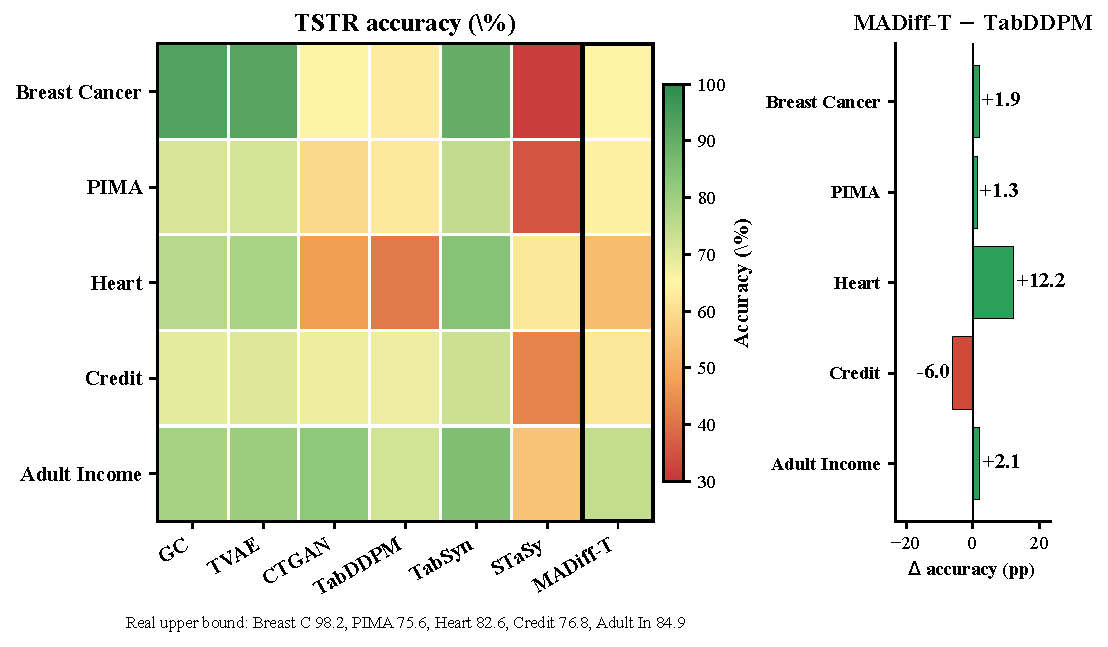
\includegraphics[width=\linewidth]{figures/comparative_utility_IS.pdf}
    \caption{Comparative downstream utility under TSTR across all datasets. Higher is better.}
    \label{fig:comparative_utility}
\end{figure}

\subsection{Fidelity and Diversity}\label{sec:results_fidelity}
We complement TSTR utility with fidelity and diversity diagnostics in Fig.~\ref{fig:fidelity_analysis}. The figure summarizes (i) marginal distribution alignment (continuous and categorical features) and (ii) correlation-structure similarity between real and synthetic data.

\noindent\textit{Practical implication:} Fidelity diagnostics help interpret whether utility differences are driven by meaningful distributional alignment versus structural distortions, and should be read alongside privacy audits.

\begin{figure*}[!htpb]
    \centering  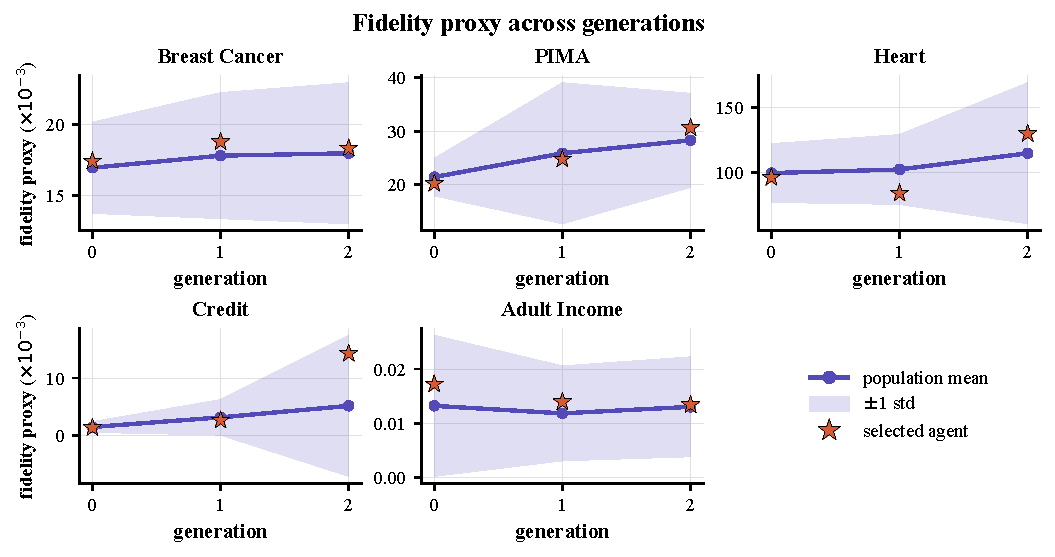
\includegraphics[width=0.84\textwidth]{figures/fidelity_analysis_IS.pdf}
    \caption{Fidelity diagnostics across all datasets across evolutionary generations 
(x-axis: generation index 0--2), summarizing the mean fidelity proxy $\pm$ std 
and the selected agent (star marker) at each generation. Lower fidelity proxy 
indicates better marginal alignment and correlation-structure similarity between 
real and synthetic data.}
    \label{fig:fidelity_analysis}
\end{figure*}

\subsection{Privacy Audits: DCR Proximity and Membership Inference}\label{sec:results_privacy}
Privacy reporting varies substantially across synthetic data studies, motivating clear, attack-aware evaluation \cite{Kindji2025, Hernandez2025, Hyrup2025}. We report two primary audits used throughout this work:
(i) DCR (distance to the closest real \emph{training} record; higher is safer), and
(ii) MIA AUC (membership inference AUROC; values closer to 0.5 indicate weaker membership distinguishability under the chosen attacker, while values significantly above 0.5 indicate elevated leakage risk; in principle values below 0.5 indicate that the attacker is anti-correlated with membership and can be inverted to achieve $1-\mathrm{AUC}$, so we treat $|\mathrm{AUC}-0.5|$ as the safety-relevant magnitude).
Following attack-focused analyses of generative models \cite{Hayes2019, ZhangMalin2022, Alshantti2025}, MADiff-T incorporates these signals during selection (privacy-in-the-loop), while authenticity-style audits can be reported as secondary analyses \cite{Alaa2022}.

\paragraph{Audit definition (implementation-consistent).}
Both DCR and the distance-based membership attacker are computed in the preprocessed representation used in our evaluation scripts. \emph{Note on DCR scaling:} in-loop selection uses NormDCR (Eq.~\ref{eq:normdcr}), i.e.\ the low-quantile DCR divided by a leave-one-out within-real reference, so values are dimensionless and comparable across datasets. The DCR values reported in Tables~\ref{tab:results_privacy_all} and figures are on the evaluation scale (raw nearest-neighbor distance in the preprocessed representation), which differs from the in-loop NormDCR by a dataset-dependent constant and is therefore directly comparable across methods on the same dataset but not across datasets.
DCR is the nearest-neighbor distance from each synthetic record to the real training set (aggregated as a mean over synthetic samples). For MIA, the attacker scores a query by its proximity to the training set and AUROC is computed for distinguishing members from non-members. In-loop selection uses members from $D_{\text{train}}$ and non-members from $D_{\text{val}}$; final reporting uses members from $D_{\text{train}}$ and non-members from $D_{\text{test}}$. MIA AUC is attacker-specific: values close to 0.5 indicate weak distinguishability \emph{for this attack}, while increases above 0.5 indicate elevated leakage risk.

\noindent\textit{Takeaway:} Privacy-in-the-loop selection \emph{biases} the search toward safer audit outcomes, but improvements are attacker- and dataset-dependent; we therefore interpret results via the joint operating points (Fig.~\ref{fig:tradeoff_scatter}) rather than claiming uniform gains.

\begin{table}[!t]
\centering
\caption{Privacy audits across all datasets. Higher DCR is safer; MIA AUC closer to 0.5 indicates weaker membership distinguishability under the chosen attacker.}
\label{tab:results_privacy_all}
\scriptsize
\setlength{\tabcolsep}{5.5pt}
\renewcommand{\arraystretch}{1.15}
\rowcolors{2}{gray!10}{white}
\begin{tabular}{l|c c|c c}
\rowcolor{gray!20}
\textbf{Dataset} &
\multicolumn{2}{c|}{\textbf{TabDDPM}} &
\multicolumn{2}{c}{\textbf{MADiff-T (ours)}} \\
\rowcolor{gray!20}
& DCR $\uparrow$ & MIA AUC $\downarrow$ & DCR $\uparrow$ & MIA AUC $\downarrow$ \\
\hline
Breast Cancer & 9.09 & 0.473 & \textbf{11.06} & \textbf{0.451} \\
PIMA          & 0.49 & 0.557 & \textbf{0.53}  & \textbf{0.544} \\
Heart         & 3.09 & 0.551 & \textbf{3.57}  & \textbf{0.442} \\
Credit        & 0.73 & 0.569 & \textbf{1.93}  & \textbf{0.482} \\
Adult Income  & 0.45 & 0.486 & \textbf{1.74}  & 0.500          \\
\end{tabular}
\end{table}

Figure~\ref{fig:privacy_audits} reports DCR and MIA AUC across all datasets and methods. The audits can disagree across datasets and methods: for example, Adult Income shows MADiff-T with higher DCR but also slightly elevated MIA AUC, illustrating that proximity-based and membership-based audits do not always move in the same direction. This underscores the importance of reporting multiple signals and interpreting privacy as attacker-dependent rather than as a single scalar.
% --- DOMIAS (NEW) ---
\paragraph{DOMIAS membership inference audit.}
To complement the distance-based MIA proxy used in-loop, we additionally report DOMIAS AUC \cite{vanbreugel2023domias_aistats}, computed using members from $D_{\text{train}}$ and non-members from $D_{\text{test}}$ under the standard DOMIAS protocol. Lower AUC is safer; values close to 0.5 indicate chance-level membership distinguishability under this attacker.
\begin{table}[!t]
\centering
\caption{DOMIAS membership-inference AUC for MADiff-T
($M=6$, seeded; mean $\pm$ std over 5 seeds; members $D_{\text{train}}$,
non-members $D_{\text{test}}$) under the standard DOMIAS protocol \cite{vanbreugel2023domias_aistats}. Values closer to 0.5 indicate weaker
membership distinguishability under this attacker. Reported as a
secondary diagnostic complementing the in-loop distance-based MIA
audit; all values near 0.5 indicate low membership leakage risk.}
\label{tab:results_domias}
\scriptsize
\setlength{\tabcolsep}{5.5pt}
\renewcommand{\arraystretch}{1.15}
\rowcolors{2}{gray!10}{white}
\begin{tabular}{l|c}
\rowcolor{gray!20}
\textbf{Dataset} & \textbf{MADiff-T DOMIAS AUC $\downarrow$} \\
\hline
Adult Income  & 0.498 $\pm$ 0.002 \\
Breast Cancer & 0.448 $\pm$ 0.030 \\
German Credit & 0.476 $\pm$ 0.047 \\
Heart Disease & 0.487 $\pm$ 0.043 \\
PIMA Diabetes & 0.557 $\pm$ 0.017 \\
\end{tabular}
\end{table}

\begin{figure*}[!htpb]
    \centering
    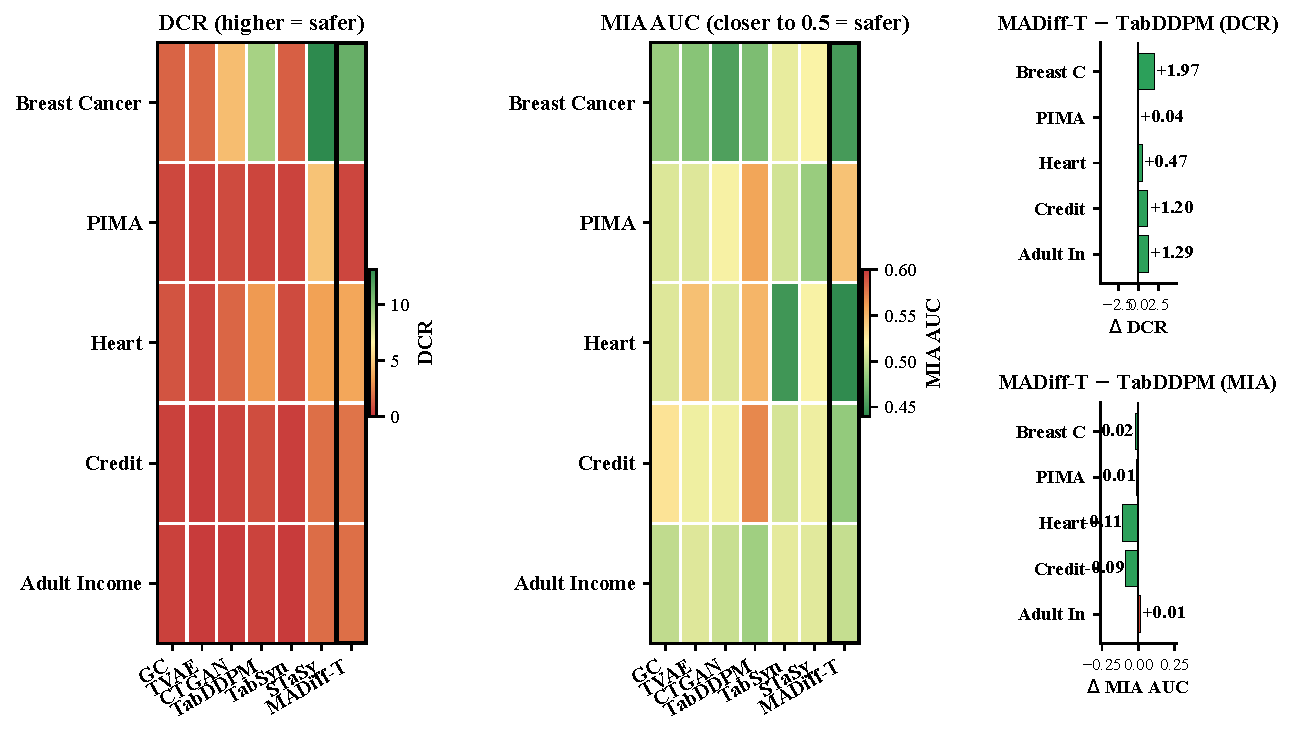
\includegraphics[width=\textwidth]{figures/privacy_audits_IS.pdf}
    \caption{Privacy audits across all datasets: DCR (higher is safer) and MIA AUC (closer to 0.5 indicates weaker membership distinguishability under the chosen attacker).}
    \label{fig:privacy_audits}
\end{figure*}

\begin{figure}[!htpb]
    \centering
    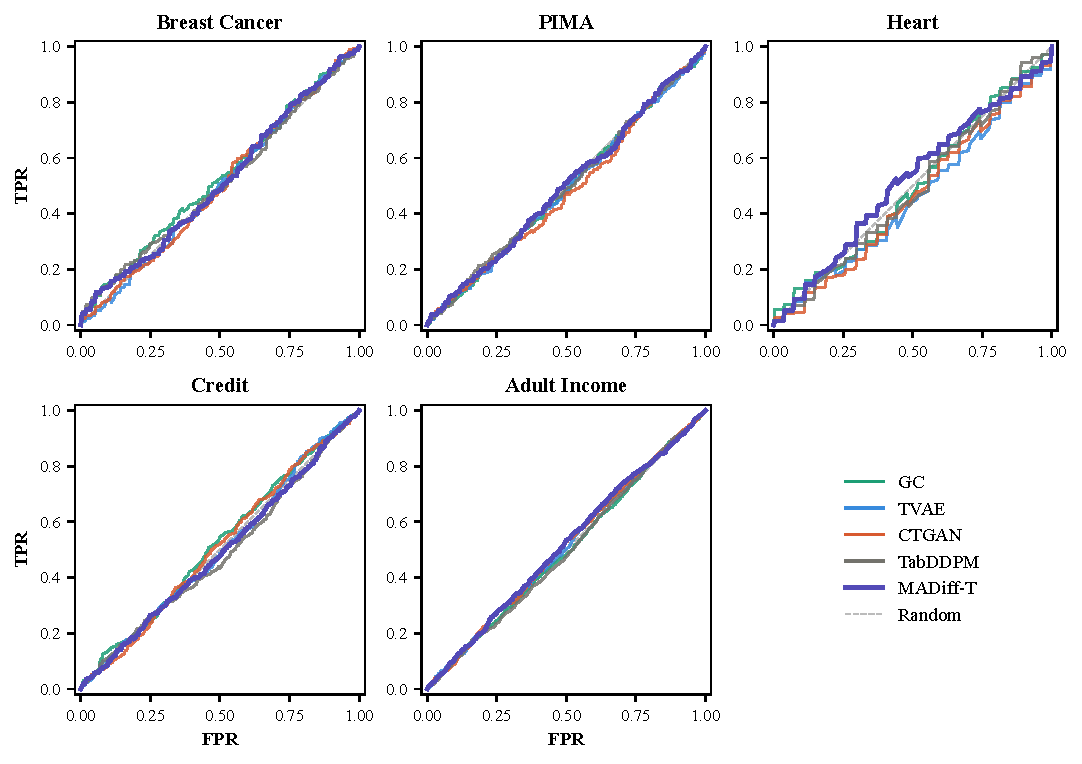
\includegraphics[width=\textwidth]{figures/mia_roc_curves_IS.pdf}
    \caption{ROC curves for the distance-based membership inference attacker (mean over 5 seeds). All methods cluster near the diagonal, indicating near-chance membership distinguishability. The MADiff-T curve (thick) tracks close to the TabDDPM baseline, consistent with the scalar MIA AUC values in Table~\ref{tab:results_privacy_all}.}
    \label{fig:mia_roc}
\end{figure}

\begin{figure*}[!t]
    \centering
    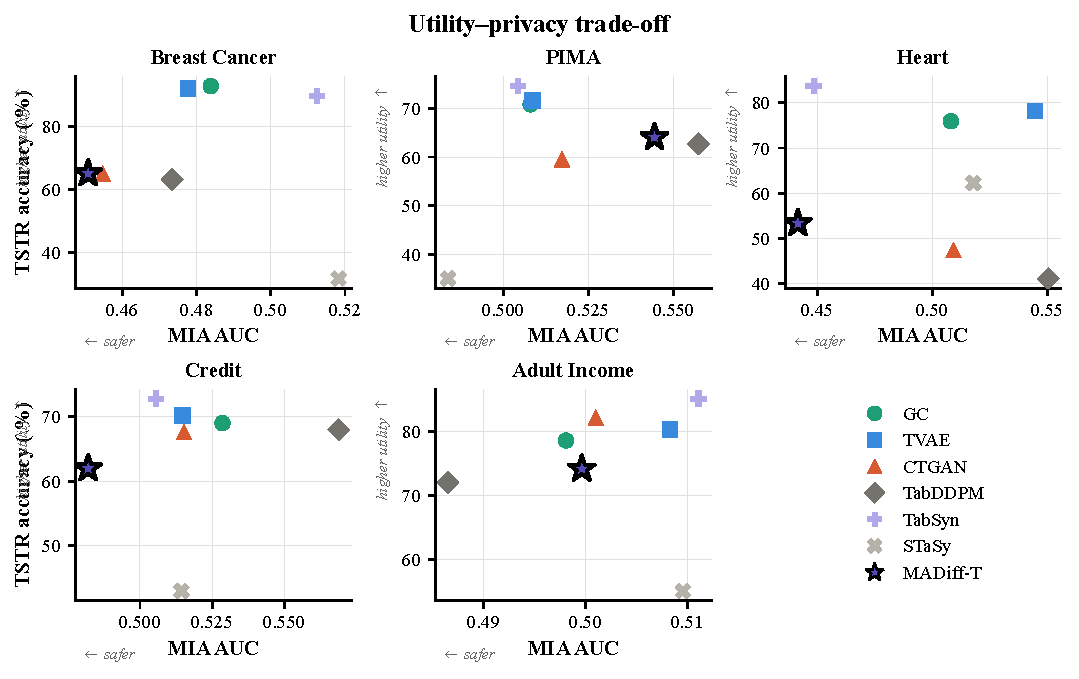
\includegraphics[width=\textwidth]{figures/tradeoff_scatter_IS.pdf}
    \caption{Utility--privacy operating points across all datasets. Better trade-offs move toward higher utility and safer privacy (higher DCR and lower MIA AUC).}
    \label{fig:tradeoff_scatter}
\end{figure*}

\subsection{Ablations and Sensitivity}\label{sec:results_ablation}
We ablate core components in two stages. Table~\ref{tab:ablation_steps} isolates the contribution of each enhancement step, comparing the original submission baseline, the addition of FA Loss (Step~1), and the full system with Per-Feature 
Schedule offsets (Step~2). Figure~\ref{fig:ablation_study} further isolates the impact of (i) removing weight inheritance, (ii) utility-only selection (privacy evaluated post hoc), and (iii) restricting mutations to optimizer parameters only.

\begin{table}[!t]
\centering
\caption{Ablation: TSTR accuracy (\%, mean $\pm$ std over 5 seeds, 
$M=6$ seeded) as enhancements are added. Original = base evolutionary 
calibration only (no FA Loss, no PFS); +FA Loss = Feature-Aggregated 
Loss added; +FA Loss+PFS = full MADiff-T. Since Final equals +FA Loss 
on all datasets where PFS is disabled, those rows are marked 
$\dagger$. PFS is active only for PIMA ($n_{\text{train}} \geq 520$, 
categorical ratio $< 0.5$).}
\label{tab:ablation_steps}
\scriptsize
\setlength{\tabcolsep}{4pt}
\renewcommand{\arraystretch}{1.15}
\rowcolors{2}{gray!10}{white}
\begin{tabular}{l|c|c|c}
\rowcolor{gray!20}
\textbf{Dataset} & \textbf{Original} & \textbf{+FA Loss} & \textbf{+FA Loss+PFS (Final)} \\
\hline
Breast Cancer$^\dagger$ & 57.54 $\pm$ 13.54 & 65.09 $\pm$ 4.82 & 65.09 $\pm$ 4.82 \\
Adult Income$^\dagger$  & 75.23 $\pm$ 0.31  & 74.13 $\pm$ 2.09 & 74.13 $\pm$ 2.09 \\
PIMA                    & 63.51 $\pm$ 6.56  & 64.94 $\pm$ 1.89 & 64.03 $\pm$ 3.30 \\
Heart$^\dagger$         & 48.52 $\pm$ 10.67 & 53.33 $\pm$ 16.64 & 53.33 $\pm$ 16.64 \\
Credit$^\dagger$        & 55.90 $\pm$ 17.29 & 62.00 $\pm$ 12.39 & 62.00 $\pm$ 12.39 \\
\end{tabular}
\end{table}
\paragraph{Population size sensitivity.}
Table~\ref{tab:pop_sensitivity} reports the effect of population 
size on Heart Disease and German Credit, the two datasets where 
the seeded $M=4$ configuration produced results below the 
TabDDPM baseline. With $M=4$ and deterministic seeding, Heart 
TSTR falls to 36.7\% (vs.\ TabDDPM 47.4\%), showing that a 
small population can converge to a suboptimal calibration under 
a single fixed seed trajectory. Increasing to $M=6$ restores 
Heart above baseline (53.3\%), and simultaneously achieves 
the strongest membership-inference resistance in this study: 
MIA AUC on Heart falls from 0.519 (TabDDPM) to 0.442 
(MADiff-T, $M=6$). On German Credit, $M=6$ recovers 62.0\% 
versus 50.5\% for $M=4$ seeded, while also substantially 
improving both DCR (0.74$\to$1.93) and MIA AUC 
(0.560$\to$0.482). These results motivate $M=6$ as the 
default: larger populations provide more calibration diversity, 
reducing sensitivity to individual initialisation trajectories 
while weight inheritance keeps the additional compute modest.
\begin{table}[!t]
\centering
\caption{Population size sensitivity on the two datasets most 
affected by initialisation under the seeded protocol. M=6 
recovers Heart above the TabDDPM baseline and achieves 
the strongest MIA AUC improvement observed in this study 
(0.519 $\to$ 0.442). M=6 is the default for all final results.}
\label{tab:pop_sensitivity}
\scriptsize
\setlength{\tabcolsep}{3.5pt}
\renewcommand{\arraystretch}{1.15}
\begin{tabular}{l|c|c|c|c}
\toprule
\rowcolor{gray!20}
\textbf{Dataset} & \textbf{Config} & 
\textbf{TSTR (\%)} & 
\textbf{DCR $\uparrow$} & 
\textbf{MIA AUC $\downarrow$} \\
\midrule
\multirow{3}{*}{Heart}
 & TabDDPM (baseline) 
   & 47.41 $\pm$ 15.96 & 2.85 & 0.519 \\
 & MADiff-T $M=4$ (seeded) 
   & 36.67 $\pm$ 5.46  & 3.28 & 0.481 \\
 & MADiff-T $M=6$ (seeded, final) 
   & \textbf{53.33 $\pm$ 16.64} & \textbf{3.57} & \textbf{0.442} \\
\midrule
\multirow{3}{*}{German Credit}
 & TabDDPM (baseline) 
   & 70.30 $\pm$ 0.76  & 0.74 & 0.560 \\
 & MADiff-T $M=4$ (seeded) 
   & 50.50 $\pm$ 17.73 & 2.05 & 0.522 \\
 & MADiff-T $M=6$ (seeded, final) 
   & \textbf{62.00 $\pm$ 12.39} & \textbf{1.93} & \textbf{0.482} \\
\bottomrule
\end{tabular}
\end{table}
\noindent\textit{Takeaway:} FA Loss provides the largest utility
contribution on most datasets (e.g., $+$7.6pp on Breast Cancer,
$+$4.8pp on Heart vs.\ no-FA-Loss baseline) and should be regarded
as the primary training enhancement introduced in this work. PFS
is better understood as an optional extension: under the adaptive
rule it is active only on PIMA among our benchmarks, where it
contributes a small privacy-guided recalibration on top of FA Loss.
On the remaining datasets PFS is frozen at zero and +FA Loss+PFS
coincides exactly with +FA Loss (marked $\dagger$ in
Table~\ref{tab:ablation_steps}); PFS is therefore most useful as
a targeted extension for larger, predominantly-continuous datasets
rather than a universally-on component. Population size materially affects 
result stability under deterministic seeding: $M=6$ is recommended 
as the minimum for reliable calibration search on small datasets. 
Regarding the Adult Income exception in Table~\ref{tab:ablation_steps}, +FA Loss reduces TSTR marginally relative to 
the no-loss baseline (74.13\% vs.\ 75.23\%), consistent with 
the known behaviour of inverse-variance weighting on 
low-variance continuous features where the reweighting 
redistributes gradient signal away from already well-learned 
features; the privacy operating point nonetheless improves.

\begin{figure*}[!t]
    \centering
    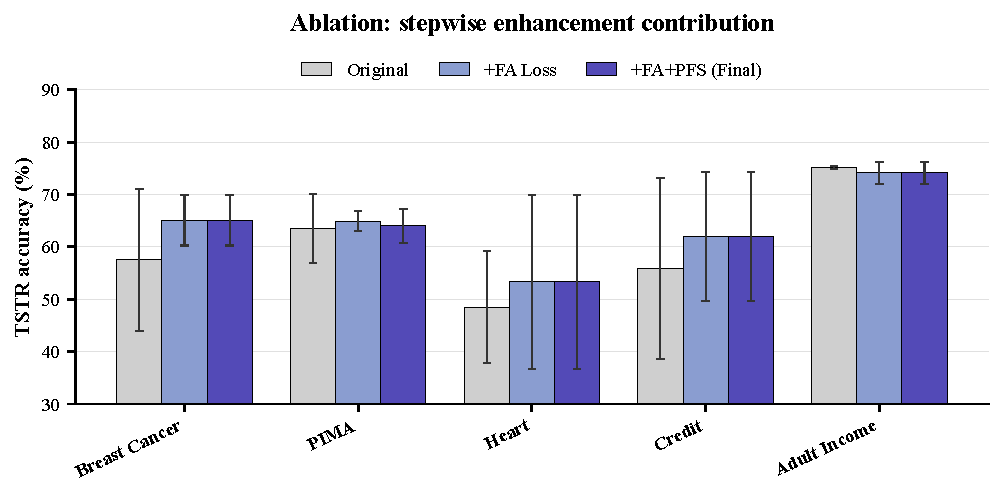
\includegraphics[width=\textwidth]{figures/ablation_study_IS.pdf}
    \caption{Ablation study: impact of core MADiff-T components on utility and privacy metrics across datasets.}
    \label{fig:ablation_study}
\end{figure*}

\begin{figure}[!t]
    \centering
    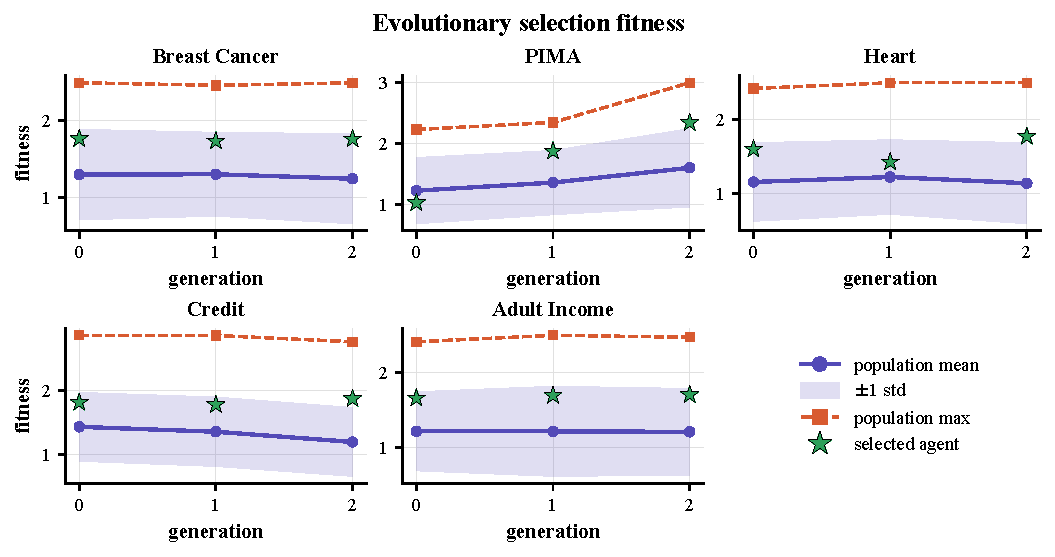
\includegraphics[width=.9\textwidth]{figures/evolution_curves_IS.pdf}
    \caption{Evolution of MADiff-T selection fitness across generations for all datasets.}
    \label{fig:evolution_curves}
\end{figure}

\subsection{Compute and Practical Considerations}\label{sec:results_compute}
MADiff-T introduces additional compute relative to training a single diffusion model because it evaluates a population of candidates across generations. In the absence of weight inheritance, a naive implementation would scale roughly as $M \cdot G$ times the cost of a single TabDDPM run ($M=6$ agents across $G$ generations). Weight inheritance reduces this overhead substantially by reusing learned parameters across generations, so each child agent requires only a short fine-tuning step per mutation rather than a full retrain; in practice, the effective overhead is closer to the cost of training $M$ single models with short refinement passes, not $M \cdot G$ full retrains. Per-run wall-clock logs and hardware details are provided in the released bundle (see \texttt{compute\_summary.csv}).

\subsection{Summary of Findings}\label{sec:results_summary}
Across five datasets, we jointly evaluate downstream utility (TSTR), fidelity diagnostics, and attack-aware privacy audits. MADiff-T is most appropriately evaluated by its \emph{operating point}: privacy-in-the-loop selection biases the search toward candidates with improved audit outcomes when utility is comparable, while acknowledging that privacy gains are not uniform across datasets or attackers. Overall, our results show that incorporating privacy audits during model selection can shift utility--privacy trade-offs without large utility collapse relative to a strong single-model diffusion baseline, and that reporting utility alone is insufficient for assessing synthetic data release risk.

\section{Limitations}
MADiff-T has several limitations that are important for correct interpretation and deployment. First, our privacy findings are \emph{audit-based} rather than formal guarantees: DCR and membership-inference AUROC quantify leakage risk only under the stated protocols and attacker class (here, proximity- and distance-based attackers). Privacy signals can be \emph{dataset- and attacker-dependent} and may occasionally disagree (e.g., improved proximity with weaker resistance to a particular MIA), so our results should not be interpreted as universal protection against all adversaries or as a differential privacy guarantee. Moreover, because audits are part of the selection objective, there is a risk of \emph{overfitting to the chosen audits}: a selected model may appear safer under these metrics while not necessarily remaining robust to stronger, privacy-adaptive attackers. Second, population-based refinement incurs additional compute relative to training a single diffusion model. Although weight inheritance and parallelism can reduce wall-clock overhead, practical use may be constrained by available GPU resources, limiting population size, generations, or per-agent budgets. Third, the composite fitness compresses utility, fidelity, and privacy into a scalar score; the relative weighting and normalization determine which operating point is selected, and different applications or stakeholders may prefer different trade-offs (e.g., prioritizing privacy over utility). Finally, our evaluation focuses on standard tabular benchmarks with fixed splits and preprocessing; performance and privacy behavior may vary under domain shift, alternative encodings, different downstream tasks/classifiers, or alternative auditing protocols. 
Additionally, small datasets such as Heart Disease 
($n_{\text{train}}=189$) exhibit high variance in TSTR
(std $\pm$16.64pp) even with deterministic seeding and 
$M=6$, reflecting irreducible instability in low-data 
regimes; results on such datasets should be interpreted 
as indicative rather than definitive. Extending evaluation to additional domains and threat models (including stronger MIAs and attribute inference) is an important direction for future work. Finally, we do not compare directly to formally differentially private (DP) tabular baselines in this work: our privacy-audited selection is complementary to, not a substitute for, DP training. Integrating MADiff-T with DP-SGD-style training or privacy-constrained selection would provide formal $(\varepsilon,\delta)$ guarantees on top of the audit-based signals reported here and is a natural next step \cite{chen2025benchmarking_dp_tabular_synthesis}.

\section{Conclusion}
We presented MADiff-T, a multi-agent evolutionary refinement framework for tabular diffusion models that performs \emph{diffusion-specific calibration} (noise schedule, step budget, and feature-wise scaling) under a \emph{privacy-audited} fitness. Unlike conventional single-model tuning, MADiff-T trains a population of diffusion agents and applies elitist selection with mutation and weight inheritance, enabling more efficient exploration of calibration space without full retraining and reducing calibration brittleness in practice. Across multiple tabular benchmarks, MADiff-T shifts the \emph{utility--privacy operating point} relative to the single-agent TabDDPM baseline it calibrates, improving TSTR on four of five datasets (with several gains modest relative to seed variance) while selecting models that achieve more favorable trade-offs under the reported audits. We do not claim uniform dominance over architecturally distinct baselines (GANs, VAEs, or latent score-based models such as TabSyn); comparisons to those methods are reported for context only. Importantly, the multi-agent mechanism is used only during training; deployment uses a single selected refined model. Overall, our findings support privacy-in-the-loop calibration as a practical route to more transparent, attack-aware diffusion-based tabular synthesis, and motivate future work with stronger threat models, broader domains, and, where appropriate, integration with formal privacy mechanisms (e.g., DP training or privacy-constrained selection).
\section*{CRediT authorship contribution statement}
\textbf{Kumail Javaid:} Conceptualization, Methodology, Software, Validation, Formal analysis, Investigation, Data curation, Visualization, Writing -- original draft, Writing -- review \& editing.\\
\textbf{Yukang Cui:} Conceptualization, Supervision, Project administration, Writing -- review \& editing.\\

\section*{Declaration of competing interest}
The authors declare that they have no known competing financial interests or personal relationships that could have appeared to influence the work reported in this paper.

\section*{Data availability}
The datasets used in this study are publicly available: Breast Cancer (WDBC) \cite{BreastCancerWDBC}, Adult Income \cite{AdultIncome}, PIMA Diabetes \cite{PimaDiabetes}, Heart Disease \cite{HeartDisease}, and German Credit \cite{GermanCredit}.
The codebase, calibration configurations, evaluation scripts, and instructions to reproduce the experiments are available at:
\url{https://github.com/kumailjavaid21/madiff-t-release}
A permanent archival version of the code and experimental artifacts will be deposited on Zenodo upon publication.

\section*{Funding}
This research did not receive any specific grant from funding agencies in the public, commercial, or not-for-profit sectors.

\section*{Declaration of generative AI and AI-assisted technologies in the writing process}
The author(s) declare that no generative AI or AI-assisted technologies were used in the writing process of this manuscript.

% ==========================================================
% MANUAL BIBLIOGRAPHY (NO BibTeX)  ✅
% - Keep your existing \begin{thebibliography}{99} ... block
% - Author-year citations will work with natbib in authoryear mode
% ==========================================================

\begin{thebibliography}{99}
\bibitem{Kindji2025}
G.~C.~N. Kindji, L.~M. Rojas-Barahona, E. Fromont, and T. Urvoy,
``Tabular data generation models: An in-depth survey and performance benchmarks with extensive tuning,''
\emph{Neurocomputing}, vol.~658, p.~131655, 2025.

\bibitem{cormode2025synthetic_tabular_kdd}
G. Cormode, S. Maddock, E. Ullah, and S. Gade,
``Synthetic tabular data: Methods, attacks and defenses,''
in \emph{Proceedings of the 31st ACM SIGKDD Conference on Knowledge Discovery and Data Mining (KDD '25)},
Toronto, ON, Canada, Aug. 2025.

\bibitem{Pilgram2025}
J. Pilgram,
``Legal assessment of synthetic data used as anonymisation technique,''
\emph{Computer Law \& Security Review}, 2025.

\bibitem{Shokri2017}
R. Shokri \emph{et al.},
``Membership inference attacks against machine learning models,''
in \emph{IEEE Symposium on Security and Privacy}, 2017.

\bibitem{Goodfellow2014}
I. Goodfellow \emph{et al.},
``Generative adversarial nets,''
in \emph{Advances in Neural Information Processing Systems}, 2014.

\bibitem{Xu2019a}
L. Xu, M. Skoularidou, A. Cuesta-Infante, and K. Veeramachaneni,
``Modeling tabular data using conditional GAN,''
in \emph{Advances in Neural Information Processing Systems}, 2019.

\bibitem{Alaa2022}
A. Alaa, B. van Breugel, E. Saveliev, and M. van der Schaar,
``How faithful is your synthetic data? Sample-level metrics for evaluating and auditing generative models,''
in \emph{International Conference on Machine Learning}, 2022.

\bibitem{Dwork2014}
C. Dwork and A. Roth,
``The algorithmic foundations of differential privacy,''
\emph{Foundations and Trends in Theoretical Computer Science}, vol.~9, no.~3--4, pp.~211--407, 2014.

\bibitem{Abadi2016}
M. Abadi \emph{et al.},
``Deep learning with differential privacy,''
in \emph{ACM SIGSAC Conference on Computer and Communications Security}, 2016.

\bibitem{Kotelnikov2023}
A. Kotelnikov, D. Baranchuk, I. Rubachev, and A. Babenko,
``TabDDPM: Modelling tabular data with diffusion models,''
in \emph{International Conference on Machine Learning}, 2023.

\bibitem{Zhang2024}
H. Zhang, P. Liu, Z. Zhang, C. Yan, L. Lin, and X. Liu,
``Mixed-type tabular data synthesis with score-based diffusion in latent space,''
in \emph{International Conference on Learning Representations}, 2024.

\bibitem{Tian2024}
M. Tian, B. Chen, A. Guo, S. Jiang, and A.~R. Zhang,
``Reliable generation of privacy-preserving synthetic electronic health record time series via diffusion models,''
\emph{Journal of the American Medical Informatics Association}, vol.~31, no.~11, pp.~2529--2539, 2024.

\bibitem{karras2022edm_neurips}
T. Karras, M. Aittala, S. Laine, and T. Aila,
``Elucidating the design space of diffusion-based generative models,''
in \emph{Advances in Neural Information Processing Systems}, 2022.

\bibitem{VillaizanVallelado2025}
M. Villaiz{\'a}n-Vallelado, M. Salvatori, C. Segura, and I. Arapakis,
``Diffusion models for tabular data imputation and synthetic data generation,''
\emph{ACM Transactions on Knowledge Discovery from Data}, vol.~19, no.~6, pp.~1--32, 2025.

\bibitem{Hernandez2025}
M. Hernandez, P.~A. Osorio-Marulanda, M. Catalina, A. Loinaz, G. Epelde, and N. Aginako,
``A comprehensive evaluation framework for synthetic tabular data: Balancing fidelity, utility, and privacy,''
\emph{Frontiers in Digital Health}, vol.~7, p.~1576290, 2025.

\bibitem{DeSmetCook2024}
C. DeSmet and D.~J. Cook,
``HydraGAN: A cooperative agent model for multi-objective data generation,''
\emph{ACM Transactions on Intelligent Systems and Technology}, vol.~15, no.~3, pp.~1--21, 2024.

\bibitem{Back1996}
T. B{\"a}ck,
\emph{Evolutionary Algorithms in Theory and Practice}.
Oxford University Press, 1996.

\bibitem{Hansen2001}
N. Hansen and A. Ostermeier,
``Completely derandomized self-adaptation in evolution strategies,''
\emph{Evolutionary Computation}, vol.~9, no.~2, pp.~159--195, 2001.

\bibitem{yao2025dcr_delusion}
Z. Yao, N. Kr{\v c}o, G. Ganev, and Y.-A. de Montjoye,
``The DCR delusion: Measuring the privacy risk of synthetic data,''
\emph{arXiv preprint arXiv:2505.01524}, 2025.

\bibitem{Hayes2019}
J. Hayes, L. Melis, G. Danezis, and E. De Cristofaro,
``LOGAN: Membership inference attacks against generative models,''
in \emph{Privacy Enhancing Technologies Symposium}, 2019.

\bibitem{ZhangMalin2022}
Z. Zhang, C. Yan, and B. Malin,
``Membership inference attacks against synthetic health data,''
\emph{Journal of Biomedical Informatics}, vol.~125, p.~103977, 2022.

\bibitem{lautrup2025syntheval}
A.~D. Lautrup, T. Hyrup, A. Zimek, and P. Schneider-Kamp,
``Syntheval: A framework for detailed utility and privacy evaluation of tabular synthetic data,''
\emph{Data Mining and Knowledge Discovery}, vol.~39, no.~1, pp.~1--25, 2025.

\bibitem{chen2025benchmarking_dp_tabular_synthesis}
K. Chen, X. Li, C. Gong, R. McKenna, and T. Wang,
``Benchmarking differentially private tabular data synthesis,''
\emph{arXiv preprint arXiv:2504.14061}, 2025.

\bibitem{lautrup2024systematic_review_tabular_synthesis_csur}
A.~D. Lautrup, T. Hyrup, A. Zimek, and P. Schneider-Kamp,
``Systematic review of generative modelling tools and utility metrics for fully synthetic tabular data,''
\emph{ACM Computing Surveys}, 2024.

\bibitem{zhao2022ctabganplus_frontiers}
Z. Zhao, A. Kunar, R. Birke, and L.~Y. Chen,
``CTAB-GAN+: Enhancing tabular data synthesis,''
\emph{Frontiers in Big Data}, 2024.

\bibitem{Jia2024}
F. Jia, H. Zhu, F. Jia, X. Ren, S. Chen, H. Tan, and W.~K.~V. Chan,
``A tabular data generation framework guided by downstream tasks optimization,''
\emph{Scientific Reports}, vol.~14, p.~15267, 2024.

\bibitem{Restrepo2025}
M.~F.~D. Restrepo, B. Wollmer, F. Panse, and W. Wingerath,
``Benchmarking tabular data synthesis: Evaluating tools, metrics, and datasets on prosumer hardware,''
\emph{Data Science Journal}, vol.~24, p.~37, 2025.

\bibitem{Wang2024EvolutionaryGAN}
Y. Wang, Q. Zhang, G.-G. Wang, and H. Cheng,
``The application of evolutionary computation in generative adversarial networks: A systematic literature survey,''
\emph{Artificial Intelligence Review}, vol.~57, p.~182, 2024.
\bibitem{He2021AutoML}
X. He, K. Zhao, and X. Chu,
``AutoML: A survey of the state-of-the-art,''
\emph{Knowledge-Based Systems}, vol.~212, p.~106622, 2021.
\bibitem{Austin2021}
J. Austin, D.~D. Johnson, J. Ho, D. Tarlow, and R. van den Berg,
``Structured denoising diffusion models in discrete state-spaces,''
in \emph{Advances in Neural Information Processing Systems}, 2021.

\bibitem{Hyrup2025}
T. Hyrup, A.~D. Lautrup, A. Zimek, and P. Schneider-Kamp,
``A systematic review of privacy-preserving techniques for synthetic tabular health data,''
\emph{Discover Data}, vol.~3, p.~5, 2025.

\bibitem{vanbreugel2023domias_aistats}
B. van Breugel, H. Sun, Z. Qian, and M. van der Schaar,
``Membership inference attacks against synthetic data through overfitting detection,''
in \emph{Proceedings of the 26th International Conference on Artificial Intelligence and Statistics (AISTATS 2023)},
vol.~206, \emph{Proceedings of Machine Learning Research}, 2023.

\bibitem{Alshantti2025}
A. Alshantti, A. Rasheed, and F. Westad,
``Privacy re-identification attacks on tabular GANs,''
\emph{Security and Privacy}, vol.~8, no.~1, p.~e469, 2025.

\bibitem{houssiau2022tapas}
F. Houssiau \emph{et al.},
``TAPAS: A toolbox for adversarial privacy auditing of synthetic data,''
\emph{arXiv preprint arXiv:2211.06550}, 2022.

\bibitem{hu2022membership_inference_survey}
H. Hu, Z. Salcic, L. Sun, G. Dobbie, P.~S. Yu, and X. Zhang,
``Membership inference attacks on machine learning: A survey,''
\emph{ACM Computing Surveys}, vol.~54, no.~11s, pp.~1--37, 2022.

\bibitem{Patki2016}
N. Patki, R. Wedge, and K. Veeramachaneni,
``The synthetic data vault,''
in \emph{IEEE International Conference on Data Science and Advanced Analytics}, 2016.

\bibitem{Xu2019b}
L. Xu, M. Skoularidou, and K. Veeramachaneni,
``Synthetic data generation for tabular data with VAEs,''
Tech. Rep., MIT Laboratory for Information and Decision Systems, 2019.

\bibitem{Kim2023}
J. Kim, C. Lee, and N. Park,
``STaSy: Score-based tabular data synthesis,''
in \emph{International Conference on Learning Representations}, 2023.
\bibitem{BreastCancerWDBC}
W. N. Street, W. H. Wolberg, and O. L. Mangasarian,
``Nuclear feature extraction for breast tumor diagnosis,''
in \emph{Proceedings of the International Symposium on Electronic Imaging: Science and Technology}, 1993.
\bibitem{AdultIncome}
R. Kohavi,
``Scaling up the accuracy of naive-Bayes classifiers: A decision-tree hybrid,''
in \emph{Proceedings of the Second International Conference on Knowledge Discovery and Data Mining (KDD)}, 1996.
\bibitem{PimaDiabetes}
J. W. Smith, J. E. Everhart, W. C. Dickson, W. C. Knowler, and R. S. Johannes,
``Using the ADAP learning algorithm to forecast the onset of diabetes mellitus,''
in \emph{Proceedings of the Symposium on Computer Applications in Medical Care}, 1988.
\bibitem{HeartDisease}
R. Detrano, A. Janosi, W. Steinbrunn, M. Pfisterer, J. Schmid,
S. Sandhu, K. Guppy, S. Lee, and V. Froelicher,
``International application of a new probability algorithm for the diagnosis of coronary artery disease,''
\emph{American Journal of Cardiology}, vol.~64, no.~5, pp.~304--310, 1989.
\bibitem{GermanCredit}
H. Hofmann,
``Statlog (German Credit Data),''
\emph{UCI Machine Learning Repository}, 1994.

\end{thebibliography}

\end{document}